\documentclass{revtex4-1}%
\usepackage[T1]{fontenc}%
\usepackage[utf8]{inputenc}%
\usepackage{lmodern}%
\usepackage{textcomp}%
\usepackage{lastpage}%
\usepackage{graphicx}%
%
%
%
\begin{document}%
\normalsize%


\begin{figure}[h!]%
\centering%
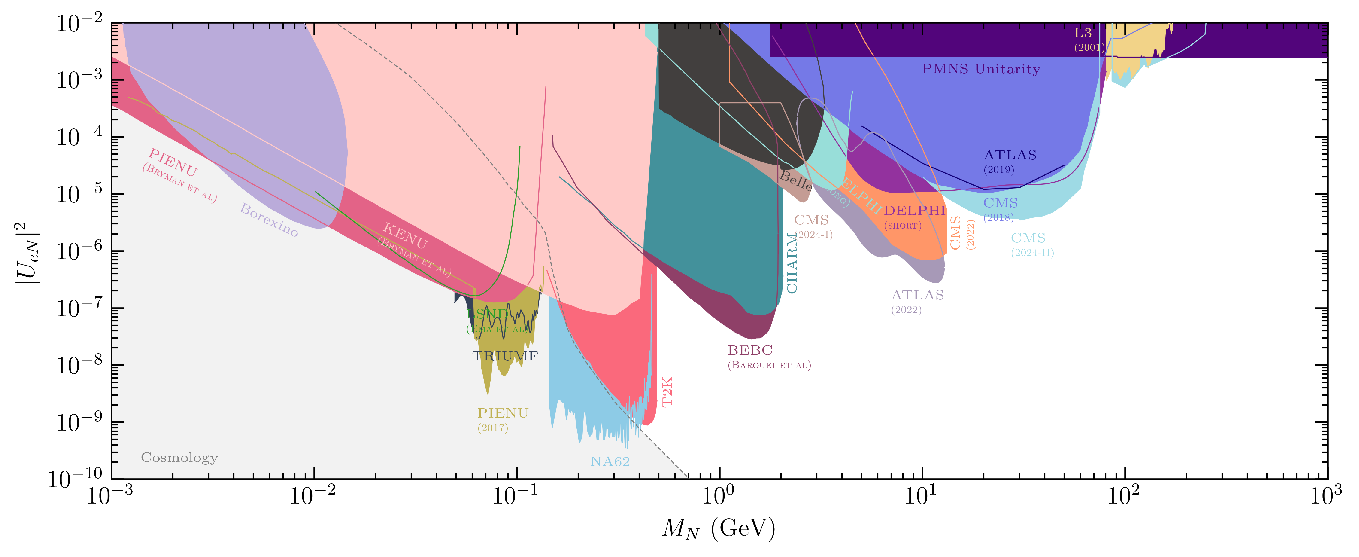
\includegraphics[width=1\textwidth]{/Users/mhostert/Repos/Heavy-Neutrino-Limits/plots/mixing/UeN_majorana.pdf}%
\caption{Constraints on $|U_{e N}|^2$ as a function of the HNL mass $m_N$. Limits shown: $K$ universality (Bryman-Shrock)~\cite{Bryman:2019bjg}, $\pi$ universality (Bryman-Shrock)~\cite{Bryman:2019bjg}, $^{20}F$ $\beta$-decay~\cite{Deutsch:1990ut}, ATLAS (2019)~\cite{ATLAS:2019kpx}, ATLAS (2022)~\cite{ATLAS:2022atq}, ATLAS (2024)~\cite{ATLAS:2024erm}, BEBC(Barouki et al)~\cite{Barouki:2022bkt}, Belle~\cite{Belle:2013ytx}, Borexino~\cite{Borexino:2013bot}, CHARM~\cite{CHARM:1985nku}, CMS (2018)~\cite{CMS:2018iaf}, CMS (2022)~\cite{CMS:2022fut}, CMS (2024-I)~\cite{CMS:2024ake}, CMS (2024-II)~\cite{CMS:2024xdq}, Cosmology~\cite{Sabti:2020yrt}, DELPHI (long)~\cite{DELPHI:1996qcc}, DELPHI (short)~\cite{DELPHI:1996qcc}, L3 (2001)~\cite{L3:2001zfe}, LSND (Ema et al)~\cite{Ema:2023buz}, NA62~\cite{NA62:2020mcv}, PIENU (2017)~\cite{PIENU:2017wbj}, PMNS Unitarity~\cite{Blennow:2023mqx}, Super-Allowed $\beta$ decays (Bryman-Shrock)~\cite{Bryman:2019bjg}, T2K~\cite{T2K:2019jwa}, TRIUMF~\cite{Britton:1992xv}.}%
\end{figure}

%


\begin{figure}[h!]%
\centering%
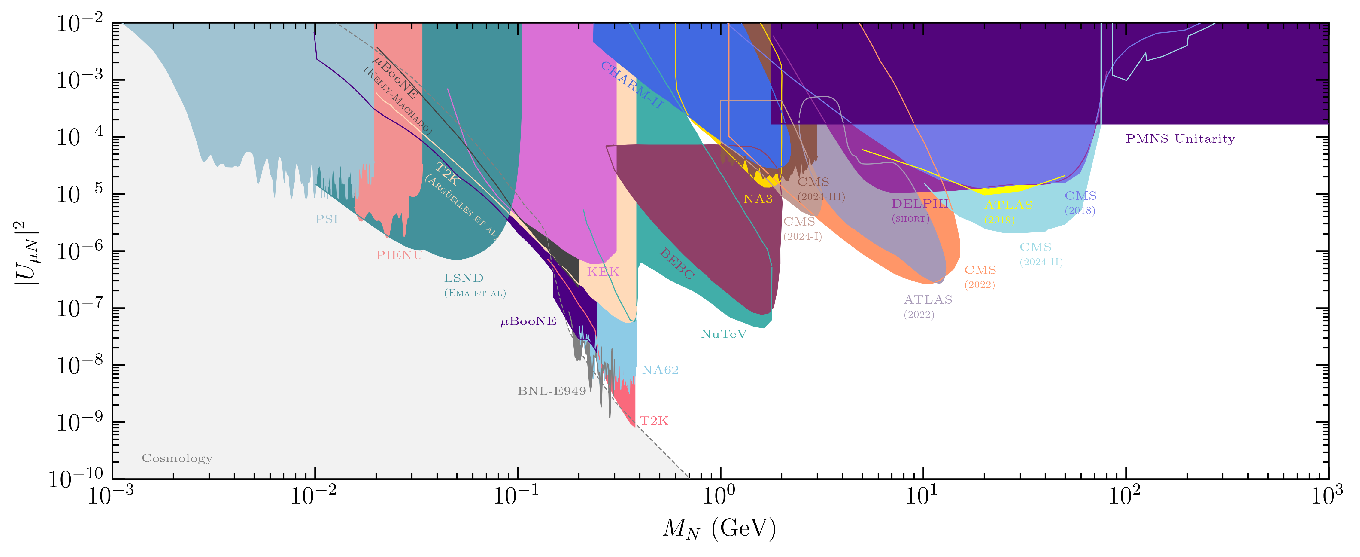
\includegraphics[width=1\textwidth]{/Users/mhostert/Repos/Heavy-Neutrino-Limits/plots/mixing/UmuN_majorana.pdf}%
\caption{Constraints on $|U_{\mu N}|^2$ as a function of the HNL mass $m_N$. Limits shown: $\mu$BooNE~\cite{MicroBooNE:2023icy}, $\mu$BooNE (Kelly-Machado)~\cite{Kelly:2021xbv}, ATLAS (2019)~\cite{ATLAS:2019kpx}, ATLAS (2022)~\cite{ATLAS:2022atq}, BEBC~\cite{WA66:1985mfx}, BNL-E949~\cite{E949:2014gsn}, CHARM-II~\cite{CHARMII:1994jjr}, CMS (2018)~\cite{CMS:2018iaf}, CMS (2018-dilepton)~\cite{CMS:2018jxx}, CMS (2022)~\cite{CMS:2022fut}, CMS (2024-I)~\cite{CMS:2024ake}, CMS (2024-II)~\cite{CMS:2024xdq}, CMS (2024-III)~\cite{CMS:2024ita}, CMS (8TeV)~\cite{CMS:2016aro}, Cosmology~\cite{Sabti:2020yrt}, DELPHI (short)~\cite{DELPHI:1996qcc}, KEK~\cite{Bryman:2019bjg}, LSND (Ema et al)~\cite{Ema:2023buz}, NA3~\cite{NA3:1986ahv}, NA62~\cite{NA62:2021bji}, NuTeV~\cite{NuTeV:1999kej}, PIENU~\cite{PIENU:2019usb}, PIENU(low $\mu$ energy)~\cite{PIENU:2019usb}, PMNS Unitarity~\cite{Blennow:2023mqx}, PSI~\cite{Daum:1987bg}, T2K~\cite{T2K:2019jwa}, T2K (Arg\"uelles et al)~\cite{Arguelles:2021dqn}.}%
\end{figure}

%


\begin{figure}[h!]%
\centering%
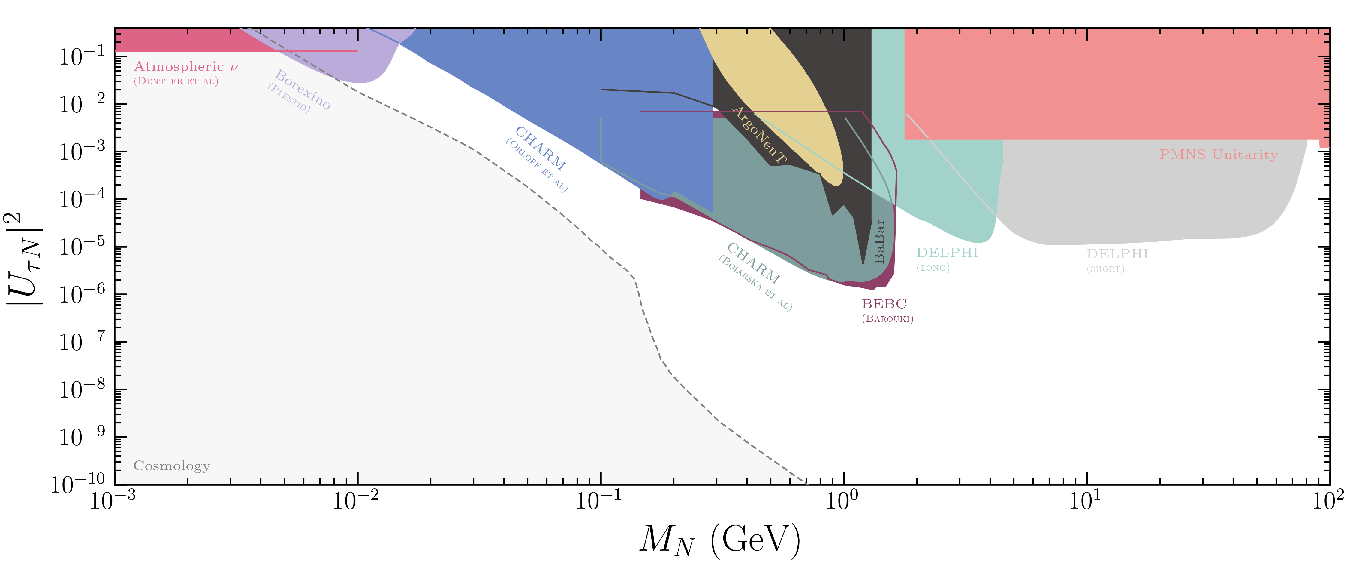
\includegraphics[width=1\textwidth]{/Users/mhostert/Repos/Heavy-Neutrino-Limits/plots/mixing/UtauN_majorana.pdf}%
\caption{Constraints on $|U_{\tau N}|^2$ as a function of the HNL mass $m_N$. Limits shown: ArgoNeuT~\cite{ArgoNeuT:2021clc}, Atmospheric $\nu$ (Dentler et al)~\cite{Dentler:2018sju}, BEBC(Barouki et al)~\cite{Barouki:2022bkt}, BaBar ~\cite{BaBar:2022cqj}, Belle~\cite{Belle:2024wyk}, Borexino (Plestid)~\cite{Plestid:2020ssy}, CHARM (Boiarska et al)~\cite{Boiarska:2021yho}, CHARM (Orloff et al)~\cite{Orloff:2002de}, CMS (2024-I)~\cite{CMS:2024ake}, CMS (2024-II)~\cite{CMS:2024xdq}, Cosmology~\cite{Sabti:2020yrt}, DELPHI (long)~\cite{DELPHI:1996qcc}, DELPHI (short)~\cite{DELPHI:1996qcc}, PMNS Unitarity~\cite{Blennow:2023mqx}.}%
\end{figure}

%
\bibliographystyle{apsrev4-1}%
\bibliography{mixing_plots}%
\end{document}